\section{磁场}\label{sec:10-2}

\begin{wrapfigure}[9]{r}{6cm}
    \centering
    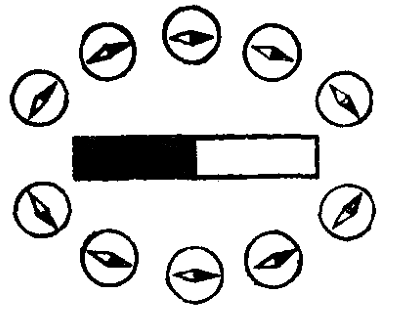
\includegraphics[width=5cm]{../pic/czwl2-ch10-8}
    \caption{}\label{fig:10-8}
\end{wrapfigure}

把一些小磁针放在条形磁铁的周围,可以看到,这些磁针静止的时候,不再指南北,
而指向新的方向(图 \ref{fig:10-8})。这是因为磁针受到了磁铁的作用力的缘故。

磁铁对磁针的作用,或者一般地说磁体间的相互作用,是怎样发生的呢?
在物理学发展的历史上,有很多学者研究过这个问题,人们经过长时期的探索和研究,
认识到磁体间的相互作用是通过磁场而发生的。
原来磁体周围的空间跟非磁体周围的空间并不相同,磁体周围的空间存在着\textbf{磁场}。
磁场虽然看不见,摸不到,我们却可以根据它所表现出来的性质来研究它。
把小磁针放在磁铁的周围,小磁针就受到磁铁的磁场的作用。
磁场的基本性质,就是它对放入其中的磁体产生磁力的作用。

磁场是有方向的。在图 \ref{fig:10-8} 中,换用别的磁针,只要放的地点不变,磁针北极所指的方向就不变。
可见,在磁场中的某一固定点,磁场对磁针北极的作用力有确定的方向。
我们把这个方向叫做这一点的磁场方向。
在磁场中的不同点,小磁针北极所指的方向不同,说明不同点的磁场方向不同。

磁场中各点的磁场方向,可以用细铁屑显示出来。

\begin{figure}[htbp]
    \centering
    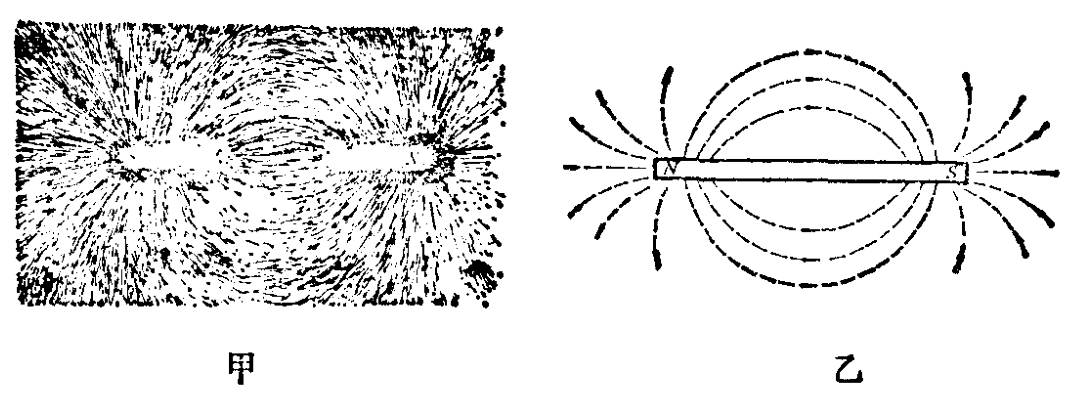
\includegraphics[width=0.8\textwidth]{../pic/czwl2-ch10-9}
    \caption{条形磁铁的磁场}\label{fig:10-9}
\end{figure}

把磁铁放在玻璃板下,在玻璃板上均匀地撒一层细铁屑。
细铁屑在磁场里被磁化成 “小磁针”,轻敲玻璃板时 “小磁针” 能在磁场作用下转动,
当它们停止下来的时候,每个 “小磁针” 的北极所指的方向就显示了它所在的那一点的磁场方向。
这无数的、分布在各个点的 “小磁针” 就显示了各个点的磁场方向,如图 \ref{fig:10-9} 甲所示。
从图中可以看出,无数的细铁屑排列成了许多条滑顺的曲线。
为了明确表示磁场的方向,这些曲线应该是有方向的:
任何一点的曲线方向都跟放在该点的磁针北极所指的方向一致。

细铁屑可以形象地显示各点的磁场方向,但是并不方便。
为了形象而又方便,我们可以仿照细铁屑的规则排列,在磁场中画一些有方向的曲线,
任何一点的曲线方向都跟放在该点的磁针北极所指的方向一致。
这的曲线叫\textbf{磁力线,磁铁周围的磁力线都是从磁铁北极出来,回到磁铁的南极}。

\begin{figure}[htbp]
    \centering
    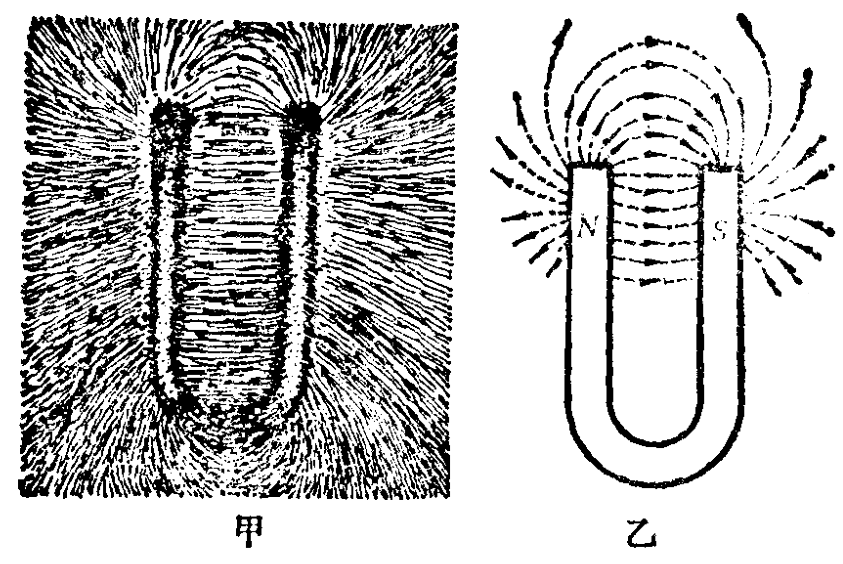
\includegraphics[width=0.7\textwidth]{../pic/czwl2-ch10-10}
    \caption{条形磁铁的磁场}\label{fig:10-10}
\end{figure}

图 \ref{fig:10-9} 乙和图 \ref{fig:10-10} 乙分别表示条形、蹄形磁铁的磁力线分布。
图 \ref{fig:10-11} 表示同名磁极间的磁场。
图 \ref{fig:10-12} 表示异名磁极间的磁场。
知道了磁场中磁力线的分布情况,就可以知道磁极在磁场中各点所受磁力的方向。
\CJKunderwave{北极在某点所受的磁力方向跟该点的磁力线方向一致,
南极所受的磁力方向跟该点的磁力线方向相反}。

\begin{figure}[H]%[htbp]
    \centering
    \begin{minipage}{7cm}
    \centering
    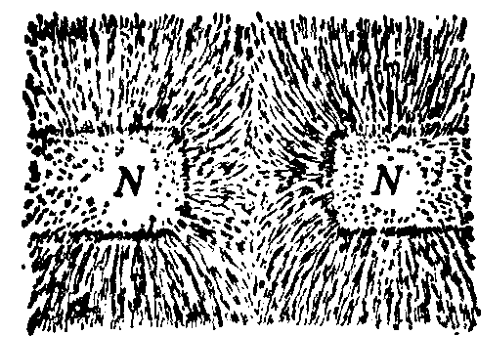
\includegraphics[width=6cm]{../pic/czwl2-ch10-11}
    \caption{同名磁极间的磁场}\label{fig:10-11}
    \end{minipage}
    \qquad
    \begin{minipage}{7cm}
    \centering
    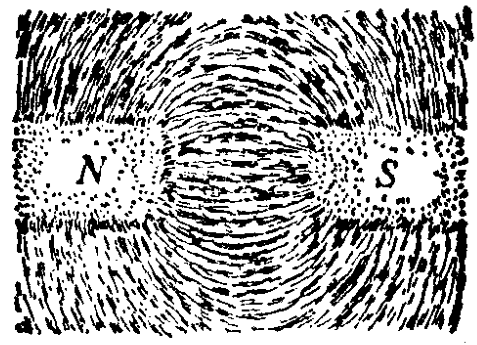
\includegraphics[width=6cm]{../pic/czwl2-ch10-12}
    \caption{异名磁极间的磁场}\label{fig:10-12}
    \end{minipage}
\end{figure}

